\documentclass[handout]{beamer}
\usepackage{tikz}
\usetikzlibrary{shapes.geometric, arrows.meta, positioning}
\tikzstyle{startstop} = [
  rectangle, rounded corners, minimum width=3cm, 
  minimum height=1cm,  text width=3cm, text centered,
  align=center, draw=black, fill=white]
\tikzstyle{arrow} = [thick, ->, >=stealth]

\usepackage{graphicx}
\usepackage{xcolor}
\usepackage{multirow}
\setbeamertemplate{blocks}[rounded][shadow=true] % estilo de bloque
\setbeamercolor{block body}{bg=gray!20, fg=black}  % fondo y texto
\setbeamercolor{block title}{bg=blue!20, fg=black} % título

%Information to be included in the title page:
\title{Aprendizaje por Refuerzo \newline
Aproximaciones}
\author{Daniela Pucci de Farias}
\institute{Universidad Torcuato Di Tella}
\date{June 2025}

\begin{document}

\frame{\titlepage}

\begin{frame}{Clase 5}
\begin{itemize}
    \item La “Maldición de la Dimensionalidad”
    \begin{itemize}
        \item MDPs de larga escala
        \item Arquitecturas de aproximación 
    \end{itemize}

\item<2-> Aplicación: Precificación de opciones
\begin{itemize}
    \item Teoría de opciones
    \item Formulación MDP y modelaje de precios de activos
    \item Simulación Monte Carlo
\end{itemize}

\end{itemize}
\end{frame}

\begin{frame}{Revisión - MDPs y Aprendizaje por Refuerzo}
\begin{center}
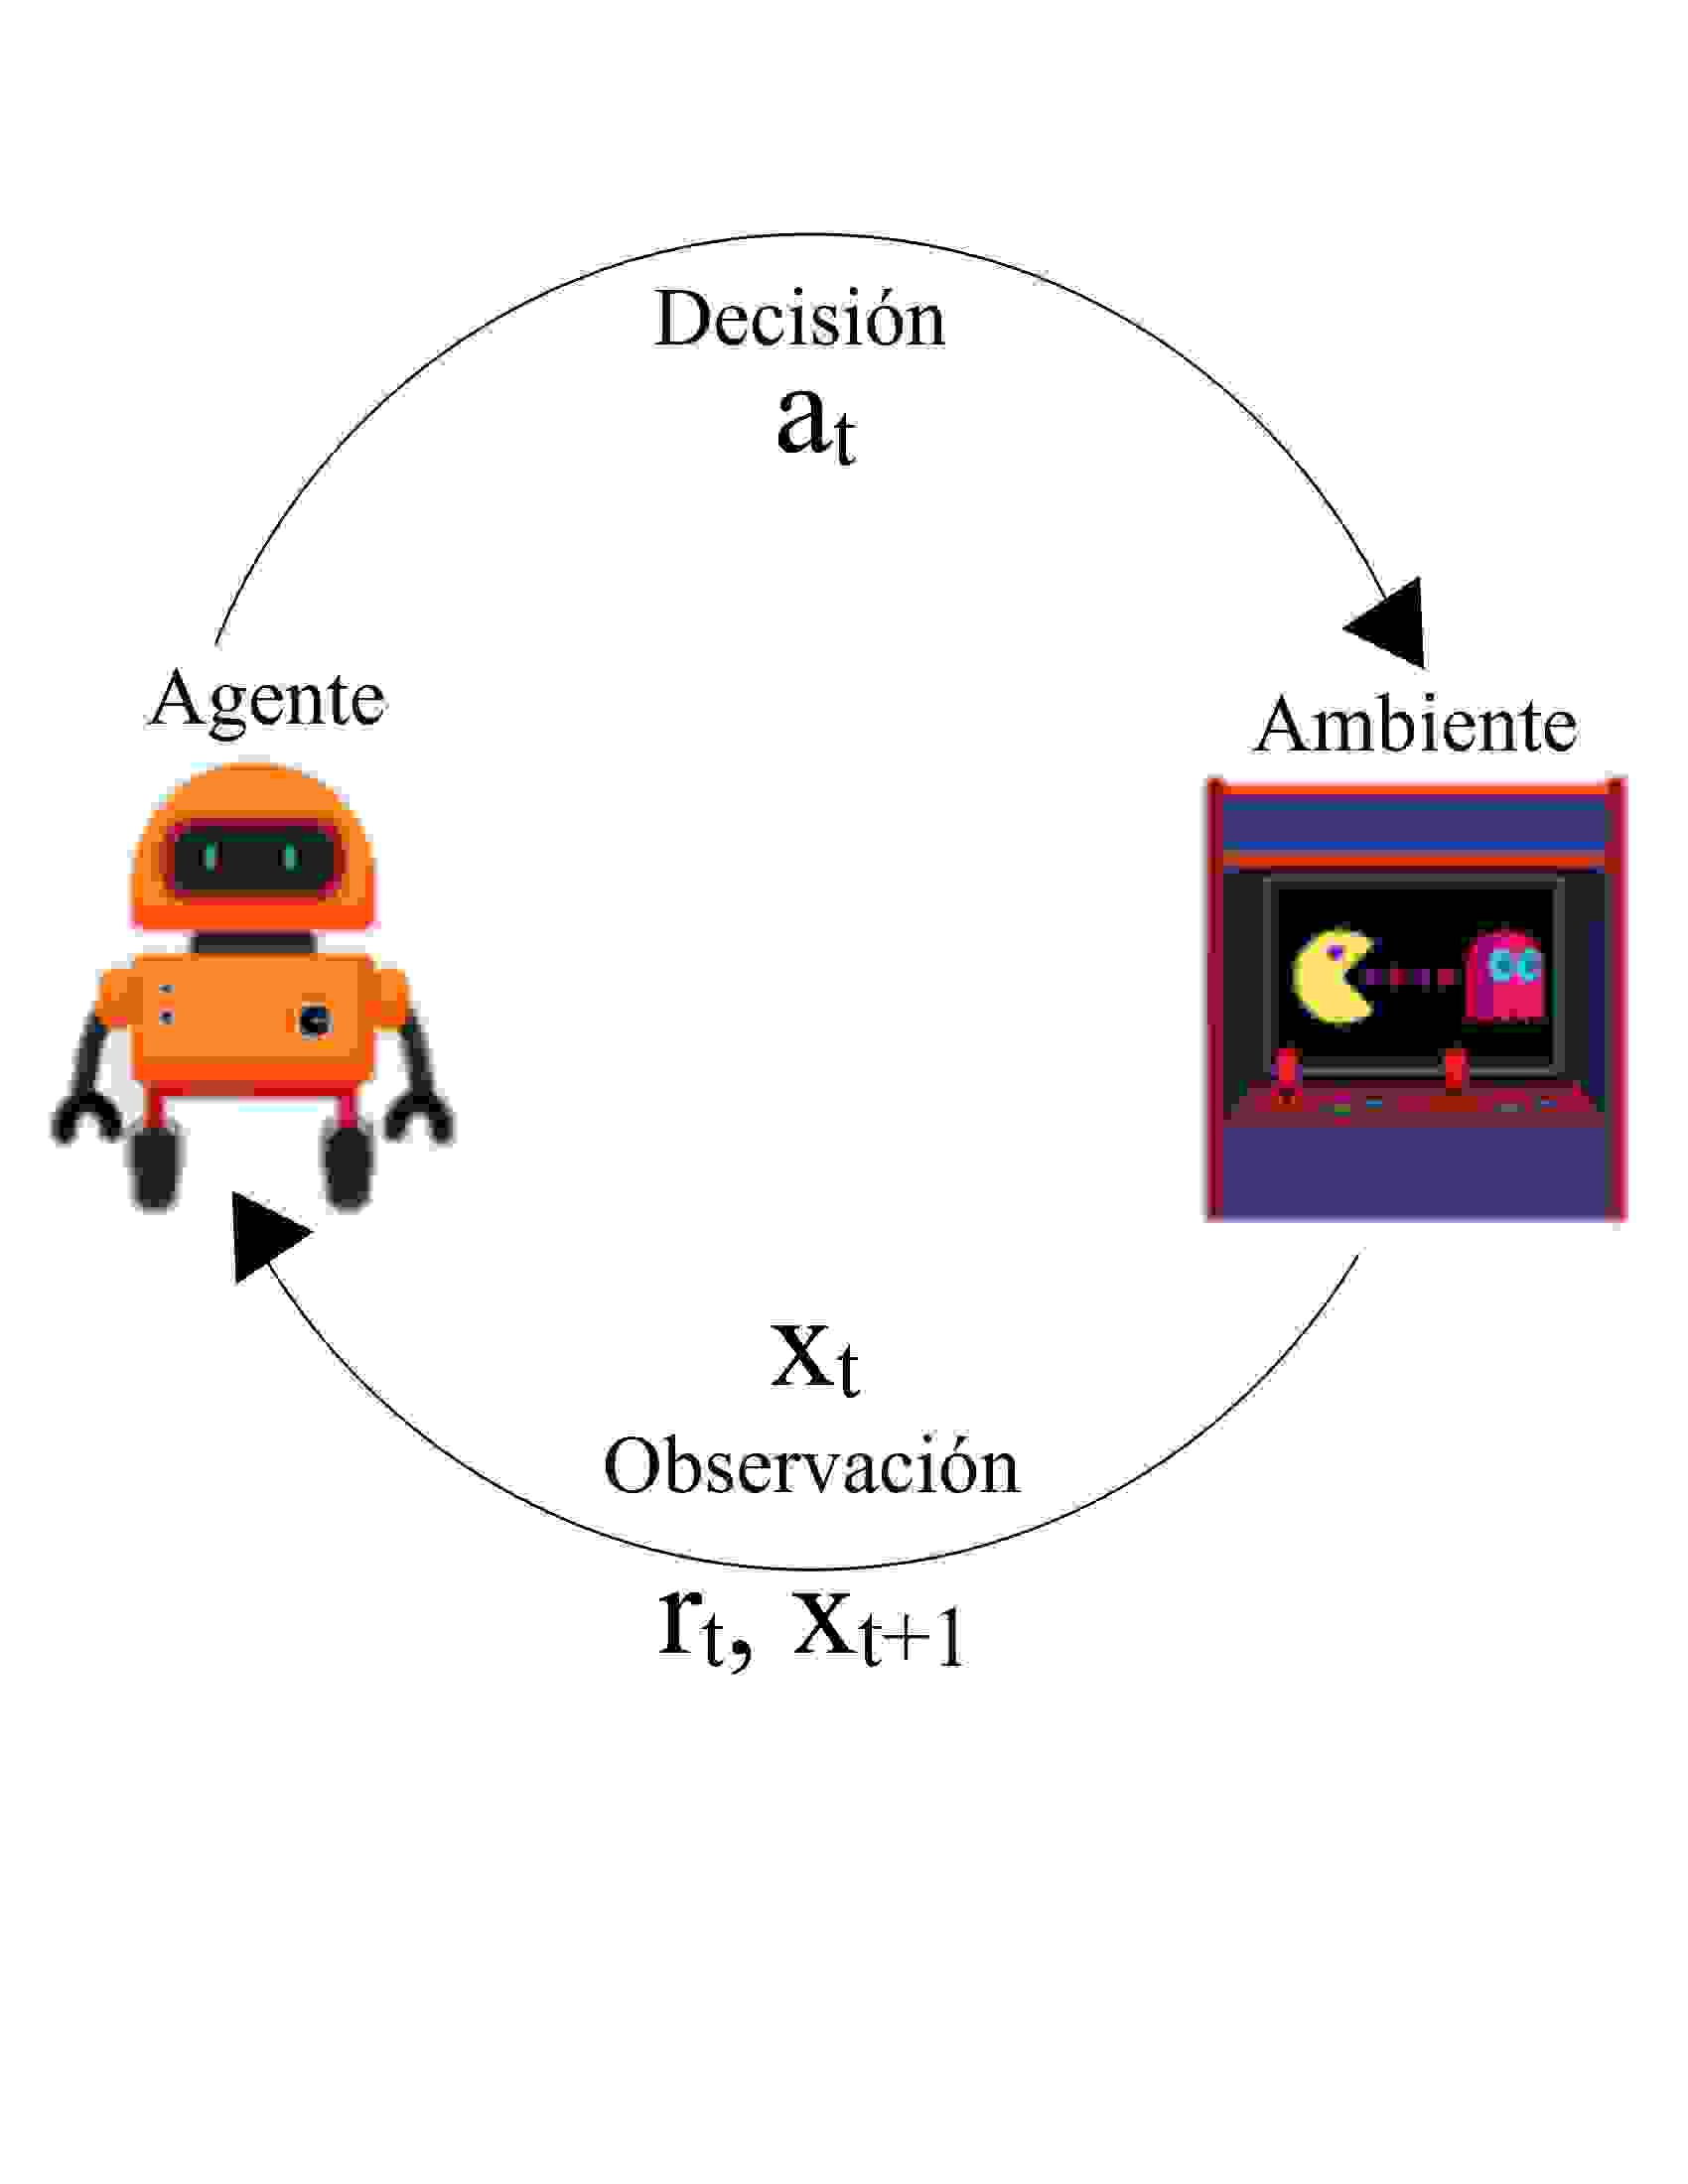
\includegraphics[width=0.5\textwidth]{../Images/Figures/LearningCycle3.jpg}
\end{center}
\vspace{-2.5cm}
\begin{columns}[t]
\hspace{1.0cm}\begin{column}{0.5\textwidth}
\begin{itemize}
    \item<3-> Agente:
    \begin{itemize}
    \item función valor $V(x)$ o $Q(x,a)$
    \item política $u(x)$
    \end{itemize}
\end{itemize}
\end{column}
\begin{column}{0.5\textwidth}
\begin{itemize}
    \item<2-> Ambiente: 
    \begin{itemize}
    \item recompensa $r_a(x)$
    \item transición $P_a(x,y)$
    \end{itemize}
\end{itemize}   
\end{column}
\end{columns}
\end{frame}

\begin{frame}{Revisión - MDPs y Aprendizaje por Refuerzo}
\begin{itemize}
\item Función valor definida por la ecuación de Bellman:
$$
\begin{array}{ccl}
V^*(x) & = &  \max\limits_{a \in A}\left\{r_a(x) + \alpha \sum_y P_a(x,y)V^*(y)\right\} \\
Q^*(x,a) & = & \left\{r_a(x) + \alpha \sum_y P_a(x,y)\max\limits_{a' \in A} Q^*(y,a')\right\}
\visible<2->{\\
V^*(x) & = & \max\limits_{a \in A} Q^*(x,a)}
\end{array}
$$
\item<3-> Resolvemos la ecuación de Bellman exactamente o con aprendizaje:
\begin{tabular}{|l|l|}
  \hline
  \textbf{Soluciones Exactas} & \textbf{Aprendizaje} \\
  \hline
\visible<4->{Iteración de valor} & \visible<4->{Simulación Monte Carlo (política fija)} \\
\visible<4->{Iteración de política} & \visible<4->{TD-Learning (política fija o variable)} \\
& \visible<5->{Q-Learning} \\
\hline
\end{tabular}
\item<6-> Calculamos la política óptima a partir de $V^*$ o $Q^*$. 
\end{itemize}
\end{frame}

\begin{frame}{Q-Learning}
\begin{block}{}
\begin{enumerate}
\item Inicializar $\hat Q$ según alguna regla y hacemos $t=1$.
\item Seleccionar acción $a^i$
\item Con observación $(x^i,a^i,r^i,y^i)$, actualizar
{\small
$$
\begin{array}{ccl}
\hat Q(x^i,a^i) & = & \hat Q(x^i,a^i) + \gamma_i\left[ r^i +\alpha \max\limits_{a \in A}\hat Q(y^i,a)-\hat Q(x^i,a^i)\right] 
\end{array}
$$}
\item Hacer $t = t+1$ y retornar al paso 2.
\end{enumerate}  
\end{block}
\begin{itemize}
\item<2-> Exploración vs exploitación: por ejemplo, elegir acción $\epsilon$-greedy.
\item<3-> Tasa de aprendizaje $\gamma_i$? Por ejemplo, $\gamma_i = 1/N_{x^i,a^i}$.
\end{itemize}
\end{frame}

\begin{frame}{La “Maldición de la Dimensionalidad”}
\begin{itemize}
\item Debemos almacenar $V^*$ o $Q^*$   
\item Tabla con un valor por estado o par estado/acción.
\item Cuánto espacio necesario?
\item<2-> Ejemplo: Ruta casa a trabajo
\begin{itemize}
\item<3-> $N$ calles norte-sur, $M$ calles este-oeste
\item<4-> Número de estados = $N \times M$
\item<4-> Número de estados/acciones
= $N \times M \times 4$
\end{itemize}
\end{itemize}
\visible<2->{
\begin{center}
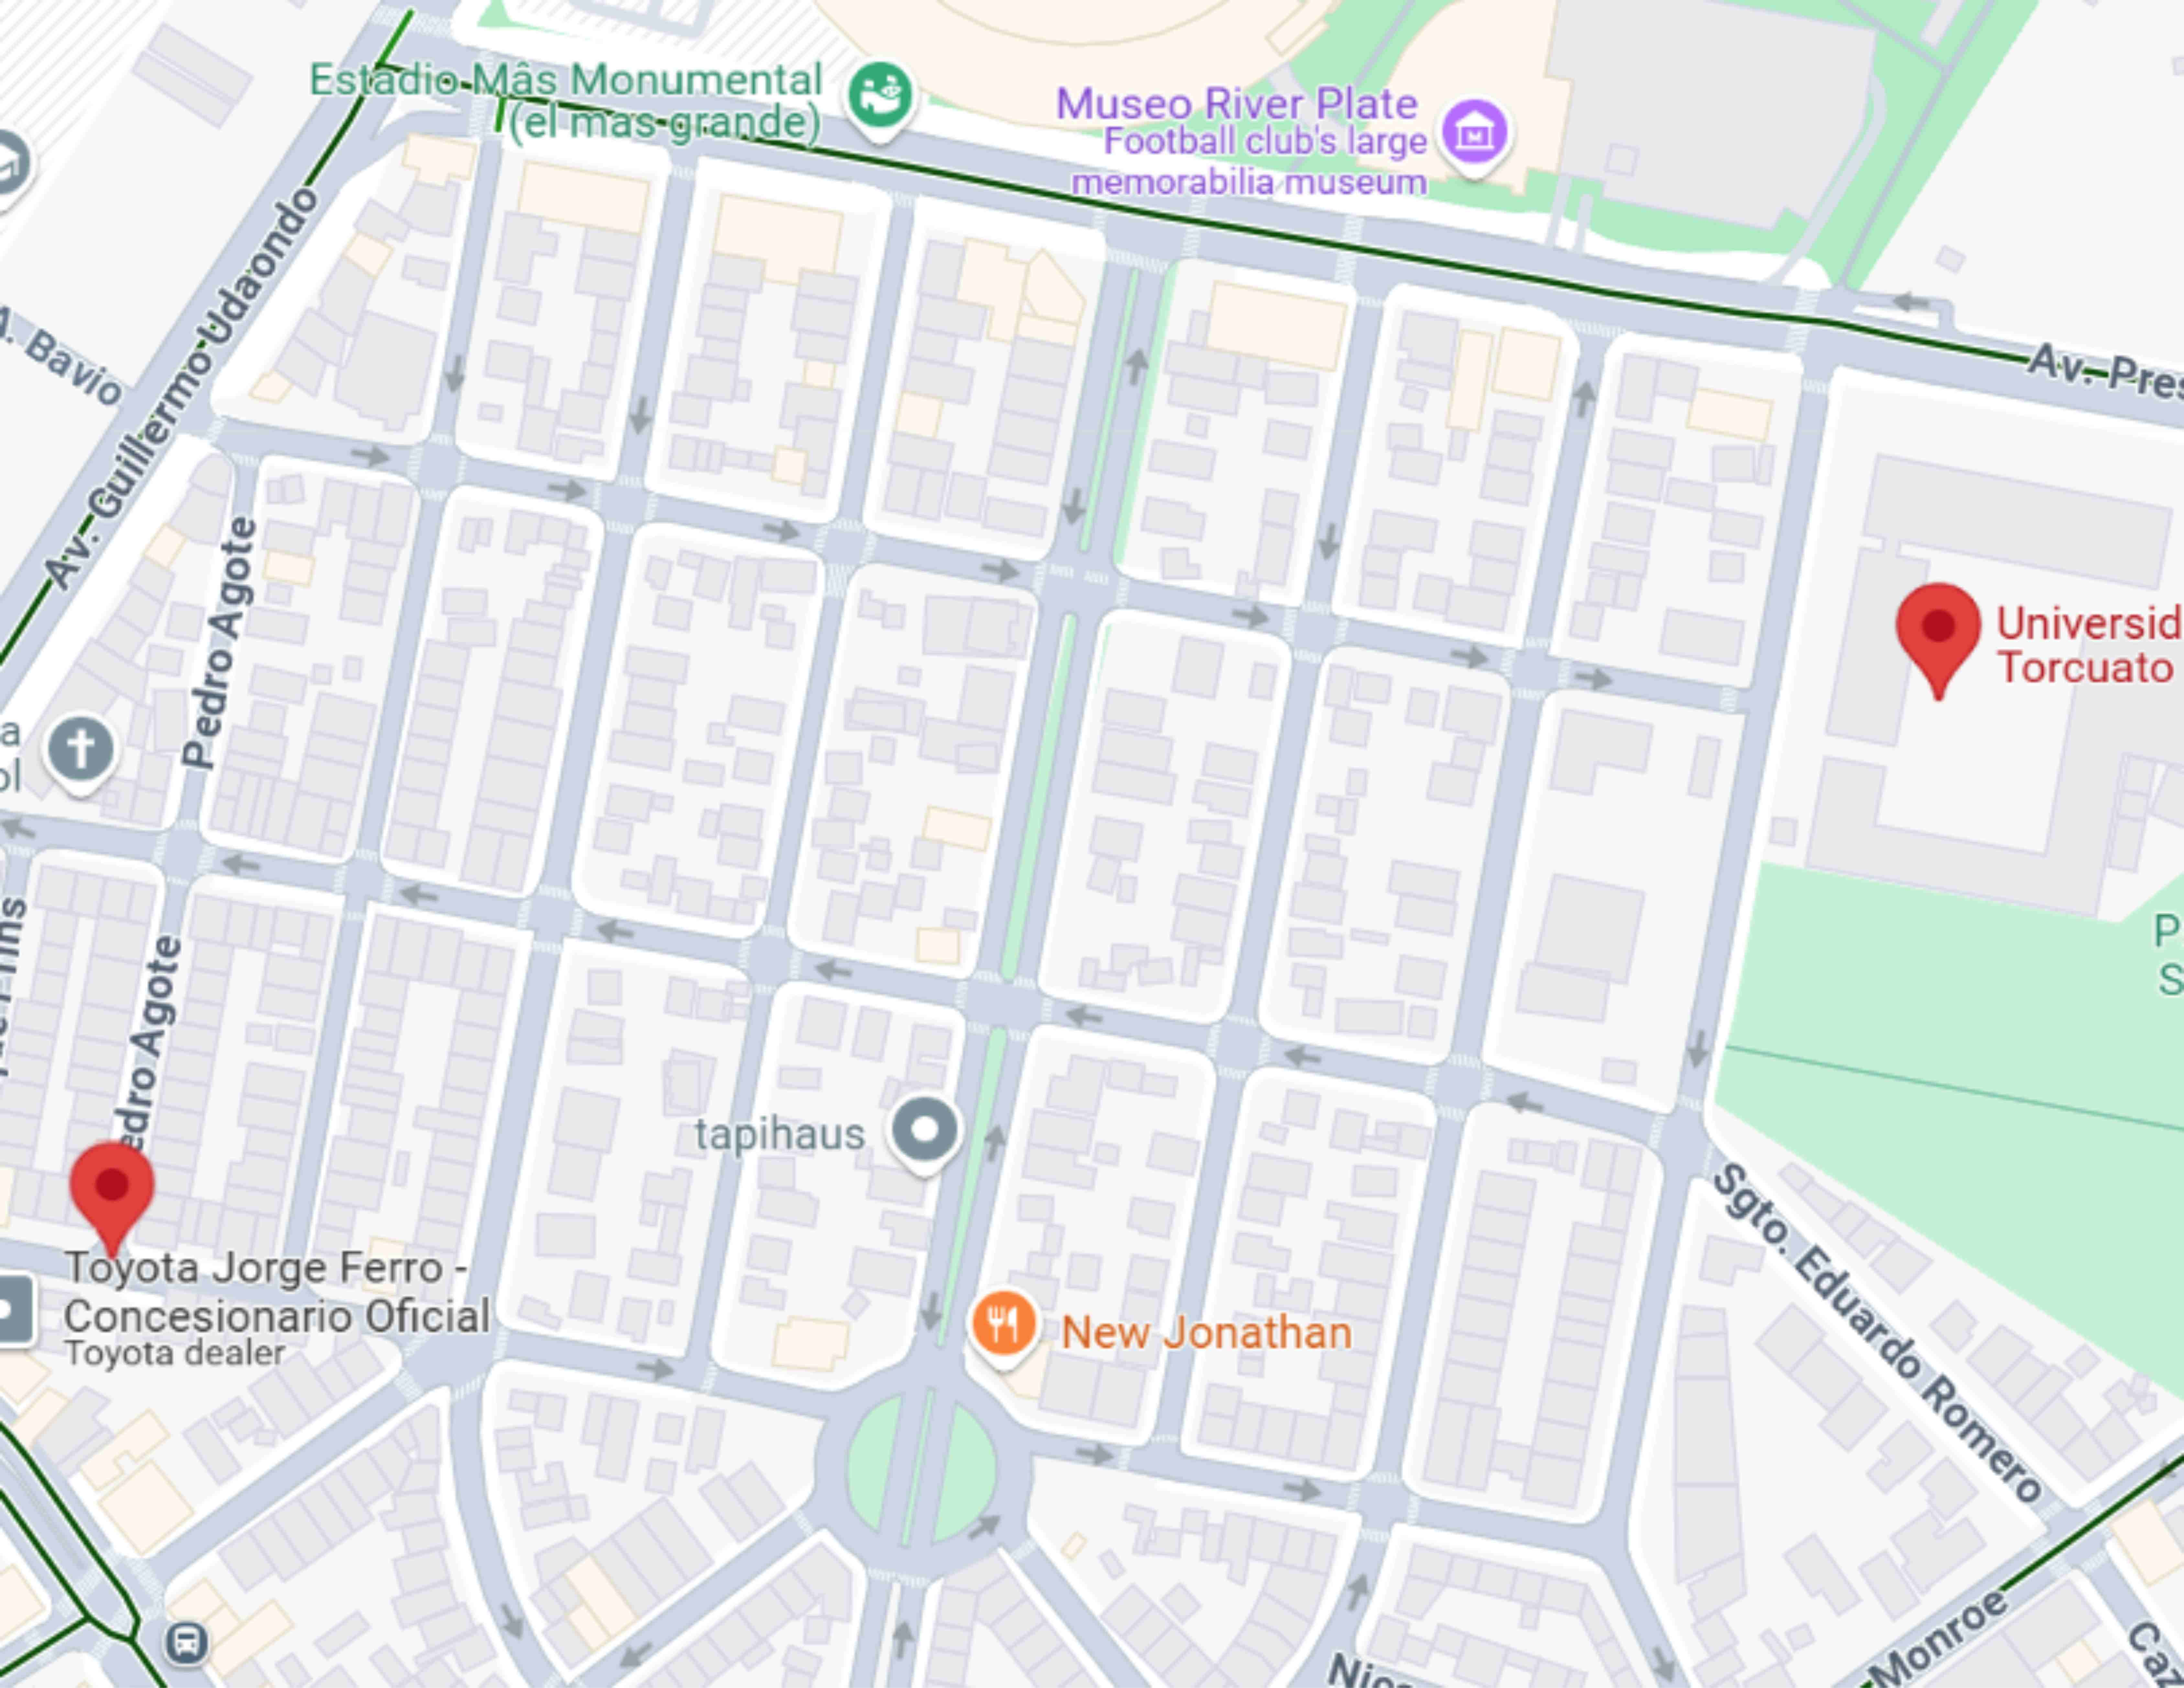
\includegraphics[width=0.5\textwidth]{../Images/Figures/mapa.jpg}
\end{center}}    
\end{frame}

\begin{frame}{La “Maldición de la Dimensionalidad”}
\begin{itemize}
\item Asumiendo $M = N$ (mapa cuadrado):
\end{itemize}
\begin{center}
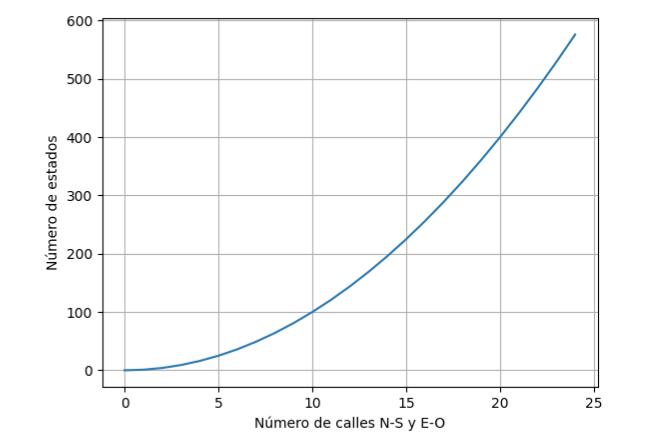
\includegraphics[width=0.8\textwidth]{../Images/Figures/NumberofStates.png}
\end{center}
\end{frame}

\begin{frame}{La “Maldición de la Dimensionalidad”}
\begin{itemize}
\item Número de estados = $N^2$
\item<2-> Crecimiento cuadrático en el número de estados con las dimensiones del grid
\item<2-> No tan dramático, porque son pocas dimensiones 
\begin{itemize}
\item<3-> Variable de estado = (i,j)
\item<3-> Variable de acción en {N, S, E, O}  
\item<3-> estado tiene 2 dimensiones, acción tiene 1
\end{itemize}
\item<4-> Nuevo problema: a cada día, una de las cuadras puede estar cortada
\begin{itemize}
\item<5-> Cómo modelar ese problema?
\item<5-> Cuántos estados?
\end{itemize}
\end{itemize}    
\end{frame}

\begin{frame}{La “Maldición de la Dimensionalidad”}
\begin{itemize}
\item Cada cuadra $c$ tiene una variable de estado con valores $\{{\rm ?, libre, cortada}\}$
\item<2-> Tenemos una variable de estado extra para cada calle
\item<3-> Estados posibles:
\begin{itemize}
\item<4-> Si aún no hemos encontrado una calle cortada:
\begin{itemize}
    \item $(c_1,c_2,\dots,c_K),~c_i \in \{{\rm }?,~{\rm libre}\}$
    \item<5-> $2^K$ estados
\end{itemize} 
\item<6-> Si ya hemos encontrado una calle cortada:
\begin{itemize}
\item<7-> $(c_1,c_2,\dots,c_n) = ({\rm libre, libre,\dots,libre, cortada, libre,\dots, libre})$ porque suponemos que hay solo una calle cortada 
\item<8-> K posibilidades
\end{itemize}
\end{itemize}
\item<9-> \textbf{El número de estados crece exponencialmente con el número de variables de estado $\rightarrow$ no podemos almacenar la función valor}
\end{itemize}
\end{frame}

\begin{frame}{Ejemplo: Go}
\begin{center}
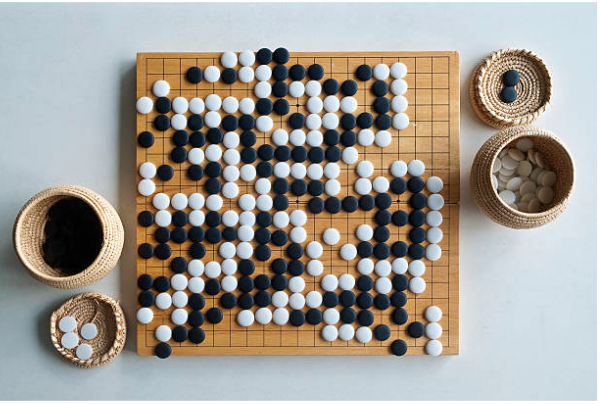
\includegraphics[width=0.8\textwidth]{../Images/Figures/Go1.png}
\end{center}
\end{frame}

\begin{frame}{Ejemplo: Go}
\begin{center}
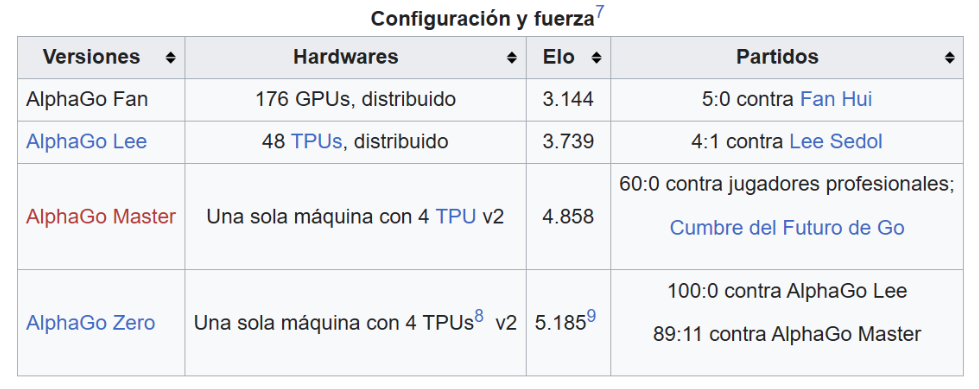
\includegraphics[width=1\textwidth]{../Images/Figures/Go2.png}
\end{center}    
\end{frame}

\begin{frame}{Ejemplo: Go - Cuántos estados?}
\begin{itemize}
\item Tablero de $19\times19$
\begin{itemize} 
\item<2-> $19 \times 19 = 361$ posiciones/variables de estado
\item<3-> cada posición puede tener 3 valores: blanco, negro, vacío
\item<4-> $3^{361} estados$ 
\item<5-> pero no todas las configuraciones son válidas
\begin{itemize}
\item<6-> aproximadamente $2.081681994 \times 10^{170}$ posiciones (2006)
\item<7-> en 2015, con avances en la potencia de computadores y nueve meses de procesamiento, John Tromp calculó el número de estados: 
\end{itemize}
\end{itemize}   
\end{itemize}
\visible<7->{
\begin{center}
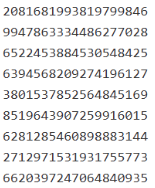
\includegraphics[width=0.3\textwidth]{../Images/Figures/Go3.png}
\end{center}}
\end{frame}

\begin{frame}{La “Maldición de la Dimensionalidad”}
\begin{itemize}
\item En la práctica, número de estados es frecuentemente prohibitivo. No podemos calcular y almacenar la función valor.
\item<2-> Solución: \textbf{generalización}
\begin{itemize}
\item Generalizar lo que sabemos sobre la función valor y o política a otros estados y acciones
\end{itemize}
\item<3-> Aproximamos la función valor y/o la función política con una \textbf{forma paramétrica}:
$$
\begin{array}{ccc}
V^*(x) \approx f(x,\theta_V),~\theta_V \in \Re^K \\ 
Q^*(x,a) \approx f(x, a, \theta_Q),~\theta_Q \in \Re^K \\
\visible<4-> {u^*(x,a) \approx f(x,a,\theta_u),~\theta_u \in \Re^K}
\end{array}
$$
\begin{itemize}
\item<5-> Es común considerar políticas randomizadas $u(x,a)$ = probabilidad de cada acción $a$ en el estado $x$ cuando aproximamos la función política.
\end{itemize}
\end{itemize}
\end{frame}

\begin{frame}{Aproximaciones Lineales}
\begin{itemize}
\item Queremos aproximar el valor de un estado \( V(x) \) sin usar una tabla
\item<2-> Usamos una combinación de funciones conocidas ("funciones básicas"):
\begin{center}
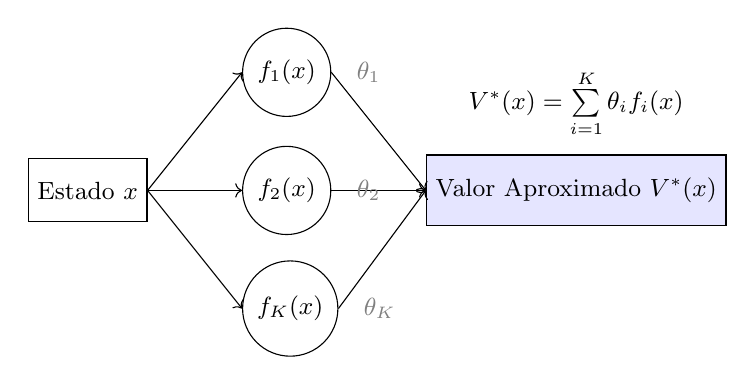
\begin{tikzpicture}[
  node distance=1.4cm and 1.2cm,
  every node/.style={font=\small},
  input/.style={draw, rectangle, minimum width=1.5cm, minimum height=0.8cm},
  func/.style={draw, circle, minimum size=1cm},
  output/.style={draw, rectangle, minimum width=2cm, minimum height=0.9cm, fill=blue!10},
  weight/.style={font=\small, gray}
]

% Nodes
\node[input] (state) {Estado $x$};

\node[func, right=of state, yshift=1.5cm] (f1) {$f_1(x)$};
\node[func, right=of state]               (f2) {$f_2(x)$};
\node[func, right=of state, yshift=-1.5cm] (fk) {$f_K(x)$};

\node[output, right=of f2] (value) {Valor Aproximado $V^*(x)$};

% Lines from state to features
\draw[->] (state.east) -- (f1.west);
\draw[->] (state.east) -- (f2.west);
\draw[->] (state.east) -- (fk.west);

% Lines from features to value
\draw[->] (f1.east) -- (value.west);
\draw[->] (f2.east) -- (value.west);
\draw[->] (fk.east) -- (value.west);
% Optional labels
\node[weight, right=0.2cm of f1] {$\theta_1$};
\node[weight, right=0.2cm of f2] {$\theta_2$};
\node[weight, right=0.2cm of fk] {$\theta_K$};
\node[above=0.1cm of value] {\small $V^*(x) = \sum\limits_{i=1}^K \theta_i f_i(x)$};
\end{tikzpicture}
\end{center}
\item<3-> Esto se llama \textbf{aproximación lineal en los parámetros} (aunque \( f_i(x) \) puede ser no lineal en $x$)
\end{itemize}
\end{frame}

\begin{frame}{Ejemplos de funciones básicas \( f_i(x) \)}
\begin{center}
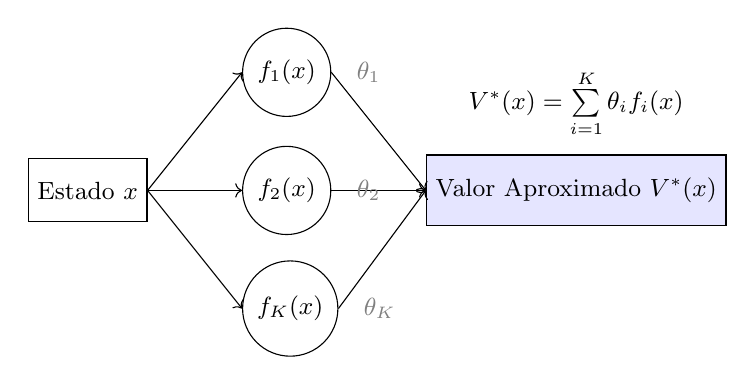
\begin{tikzpicture}[
  node distance=1.4cm and 1.2cm,
  every node/.style={font=\small},
  input/.style={draw, rectangle, minimum width=1.5cm, minimum height=0.8cm},
  func/.style={draw, circle, minimum size=1cm},
  output/.style={draw, rectangle, minimum width=2cm, minimum height=0.9cm, fill=blue!10},
  weight/.style={font=\small, gray}
]

% Nodes
\node[input] (state) {Estado $x$};

\node[func, right=of state, yshift=1.5cm] (f1) {$f_1(x)$};
\node[func, right=of state]               (f2) {$f_2(x)$};
\node[func, right=of state, yshift=-1.5cm] (fk) {$f_K(x)$};

\node[output, right=of f2] (value) {Valor Aproximado $V^*(x)$};

% Lines from state to features
\draw[->] (state.east) -- (f1.west);
\draw[->] (state.east) -- (f2.west);
\draw[->] (state.east) -- (fk.west);

% Lines from features to value
\draw[->] (f1.east) -- (value.west);
\draw[->] (f2.east) -- (value.west);
\draw[->] (fk.east) -- (value.west);
% Optional labels
\node[weight, right=0.2cm of f1] {$\theta_1$};
\node[weight, right=0.2cm of f2] {$\theta_2$};
\node[weight, right=0.2cm of fk] {$\theta_K$};
\node[above=0.1cm of value] {\small $V^*(x) = \sum\limits_{i=1}^K \theta_i f_i(x)$};
\end{tikzpicture}
\end{center}
\begin{itemize}
  \item<2-> Valores individuales de componentes del estado : \( f_i(x) = x_i \)
  \item<3-> Términos polinomiales: \( x_1^2, x_1 x_2, \dots \)
  \item<4-> Otras funciones no lineales: \( \sin(x_1), \log(x_2 + 1), \dots \)
  \item<5-> \textbf{Agregación de estados}: dividir el espacio en regiones y usar 1 o 0 según a cuál pertenece \( x \)
\end{itemize}
\end{frame}

\begin{frame}{Agregación de Estados}
 $$
f_i(x) = \begin{cases}
1 & {\rm si~} x \in S_i \\
0 & {\rm si~} x \notin S_i
\end{cases}
$$   
\begin{columns}[t]
\begin{column}[t]{0.5\textwidth}
\vspace{-4.0cm}
\begin{itemize}
\item<3-> $V^*(x) \approx V({\rm zona}(x))$
\item<4-> Buenas propiedades de convergencia
\item<5->Posibilidad de particionar espacio de 
estados progresivamente
\end{itemize}
\end{column}
\begin{column}[t]{0.5\textwidth}
\visible<2->{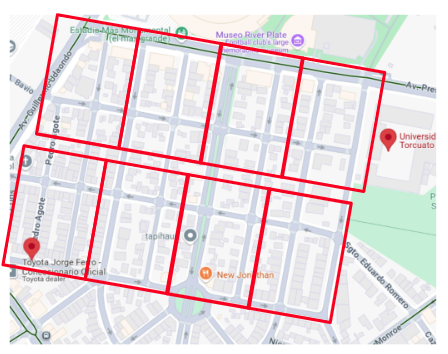
\includegraphics[width=1.0\textwidth]{../Images/Figures/StateAggregation.png}}
\end{column}
\end{columns}
\end{frame}

\begin{frame}{Aproximaciones No Lineales}
$$
V^*(x) \approx f(x,\theta)
$$
\begin{itemize}
\item $f(x,\theta)$ es no lineal en $\theta$ 
\item<2-> Ejemplo: redes neuronales
\end{itemize}
\visible<2->{
\begin{center}
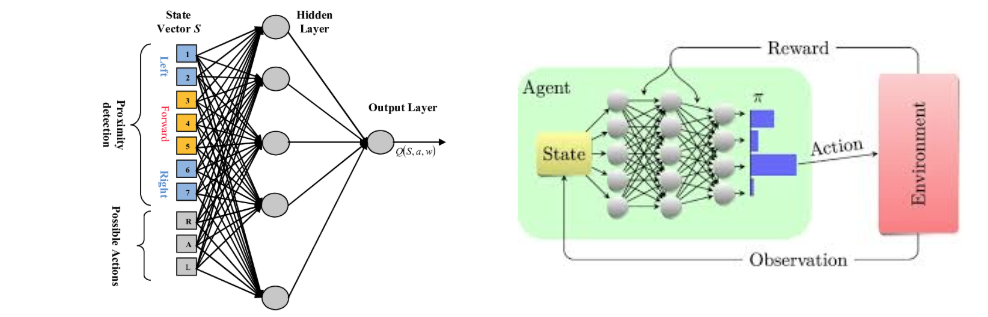
\includegraphics[width=1\textwidth]{../Images/Figures/NeuralNetwork.png}    
\end{center}}
\end{frame}

\begin{frame}{Aprendizaje Por Refuerzo Con Approximaciones}

\begin{itemize}
\item Aproximar $V^*(x) \approx f(x,\theta)$ tiene aspectos similares a aprendizaje supervisado:
\begin{itemize}
\item<2-> Tenemos pares \((x,\; y)\) y elegimos $\theta$ para que \(\hat y = f(x,\theta)\) se parezca a \(y\).  
\item<3-> Pérdida típica: \(\displaystyle\min_\theta \sum (y - f(x,\theta))^2\).
\end{itemize}
\item<4-> Pero  en RL, no hay “label” \(y\).
\item<5-> El verdadero valor $V^*(x)$ está definido implícitamente por la ecuación de Bellman:
\[
     V^*(x)=\max\limits_{a \in A}
     \left\{r_a(x)+\alpha\sum_y P_a(x,y)\,V^*(y)\right\},~\forall x.
\]
\item<6-> En vez de ajustar contra un “label”, tratamos de encontrar un valor de $\theta$ de tal forma que \(V(x,\theta)\) sea una solución aproximada a la ecuación de Bellman:  
\begin{small}
  \[
     \min_\theta \;\;\sum_x
     \underbrace{p(x)}_{\text{“peso” del estado}}\;
     \Bigl[\underbrace{\max_a\left\{r_a(x)+\alpha\sum_y P_a(x,y)V(y,\theta)\right\}-V(x,\theta)}_{\text{residuo de Bellman}}\Bigr]^2
  \]
  \end{small}
\end{itemize}
\end{frame}


\begin{frame}{Aprendizaje por Refuerzo con Aproximaciones}
\begin{itemize}
\item Queremos resolver:
\begin{small}
  \[
     \min_\theta \;\;\sum_x
     \underbrace{p(x)}_{\text{“peso” del estado}}\;
     \Bigl[\underbrace{\max_a\left\{r_a(x)+\alpha\sum_y P_a(x,y)V(y,\theta)\right\}-V(x,\theta)}_{\text{residuo de Bellman}}\Bigr]^2
  \]
  \end{small}
\item<2-> Con el espacio de estados demasiado largo, mismo conociendo $r$ y $P$ no podemos calcular el error exactamente, debemos tomar muestras
\item<3-> Aplicamos versiones de algoritmos de aprendizaje por refuerzo 
\begin{itemize}
\item<4-> Convergencia no siempre garantizada
\item<5-> Requiere técnicas de estabilización: normalización, redes objetivo, replay buffers, etc.
\item<6-> Resultados sensibles a la arquitectura y los hiperparámetros
\end{itemize}
\item<7->Ejemplos con redes neuronales:
\begin{itemize}
\item<8-> \textbf{DQN (Deep Q-Networks)}: \( Q(x,a;\theta) \) = output de red neuronal
\item<9-> \textbf{MuZero}: redes neuronales para modelo latente + valor + política
\end{itemize}
\end{itemize}
\end{frame}


\begin{frame}{Aplicación: Valuación de Opciones Americanas}
\textbf{"Opciones son instrumentos derivados que otorgan el derecho -y no la obligación-  a comprar o vender activos a un precio determinado en el contrato -denominado precio de ejercicio o strike- hasta una fecha establecida, es decir el vencimiento del contrato."}
\begin{itemize}
\item<2-> Derecho a comprar el activo = opción call
\item<3-> Derecho a vender el activo = opción put
\item<4-> Ejercicio del derecho solo en la fecha de vencimiento = \textbf{opción europea}
\item<5-> Ejercicio del derecho hasta la fecha de vencimiento = \textbf{opción americana}
\end{itemize}    
\end{frame}

\begin{frame}{Aplicación: Valuación de Opciones Americanas}
Consideramos una opción put americana, con fecha de vencimiento T y precio de ejercicio K. 
\begin{itemize}
\item<2-> Cuál debe ser el precio de la opción en t = 0?
\item<3-> Cuándo se debe ejercer la opción?   
\end{itemize}  
\end{frame}

\begin{frame}{Modelo MDP para Valuación de Opciones}
\begin{itemize}
\item Debemos definir $(S,A,P,r)$
\item<2-> Estado $s_t$ = precio del activo en el periodo $t$ 
\item<3-> Acción $a_t$ = 0 (esperar) o 1 (ejercer la opción) 
\item<4-> Recompensa $r_a(s)$:
\begin{itemize}
\item<5-> $\mathbf{r_0(s) = 0}$ (si no ejercemos, no hay recompensa inmediata) 
\item<6-> Cuánto ganamos si ejercemos la opción en en tiempo t?
\begin{itemize}
\item<7-> Compramos la acción a precio $s_t$ = precio del activo 
\item<8-> Vendemos a precio $K$
\item<9-> $\mathbf{r_1(s) = K-s}$
\end{itemize}
\end{itemize}
\item<10-> Debemos especificar $s_t$, o más generalmente la evolución de precio del activo     para terminar de definir el problema…
\end{itemize}
\end{frame}

\begin{frame}{Modelo de Precios Para Valuación de Opciones}
\begin{itemize}
\item Recordemos el modelo lognormal para precios:
$$s_{t+1} = s_t e^{r-\sigma^2/2+\sigma \epsilon_t}
$$
donde 
\begin{itemize}
\item $\epsilon_t,~t = 0,1,...$ son variables aleatorias independientes y siguen la distribución normal estándar ($\epsilon_t \sim {\rm N}(0,1)$)
\item el rendimiendo $r$ y volatilidad $\sigma$ son expresados con respeto a la duración de cada período de decision.
\end{itemize}
\item<2-> Para calcular el valor de la opción, podríamos encontrar la estragia óptima de ejercicio y evaluarla.
\item<3-> Esa solución, basada en el valor esperado, no considera el riesgo de quién vende la opción.
\item<4->Podemos aplicar la metodología modificando el modelo de precios para que sea \textbf{neutral al riesgo}.
\item<5-> Si el activo no paga dividendos, el modelo neutral al riesgo es simplemente:
$$s_{t+1} = s_t e^{r_f-\sigma^2/2+\sigma \epsilon_t}
$$
donde $r_f$ es la tasa de interés libre de riesgo.
\end{itemize}
\end{frame}

\begin{frame}{Modelo MDP para Valuación de Opciones}
\begin{itemize}
\item Debemos definir $(S,A,P,r)$
\item<2-> Estado $s_t$ = precio del activo en el periodo $t$ 
\item<3-> Acción $a_t$ = 0 (esperar) o 1 (ejercer la opción) 
\item<4-> Recompensa $r_a(s)$:
\begin{itemize}
\item<5-> $\mathbf{r_0(s) = 0}$ (si no ejercemos, no hay recompensa inmediata) 
\item<6-> Cuánto ganamos si ejercemos la opción en en tiempo t?
\begin{itemize}
\item<7-> Compramos la acción a precio $s_t$ = precio del activo 
\item<8-> Vendemos a precio $K$
\item<9-> $\mathbf{r_1(s) = K-s}$
\end{itemize}
\end{itemize}
\item<10-> Transición: 
$$s_{t+1} = s_t e^{r_f-\sigma^2/2+\sigma \epsilon_t}
$$
\item<11-> factor de descuento $\alpha = e^{-r_f}$
\end{itemize}
\end{frame}

\begin{frame}{Ecuaciones de Bellman}
\begin{itemize}
\item Cómo definir la función valor? Analizaremos la función $Q^*$.
\item<2-> El valor de ejercer la acción en cualquier periodo $t$ es conocido:
$$
Q_t^*(s,1) = K-s,~\forall t
$$
\item<3-> Podemos escribir las ecuaciones para el valor de no ejercer en el periodo actual ($a=0$) en cada periodo $t<T$:
$$
\begin{array}{ccl}
Q_t^*(s,0) & = & \alpha {\rm E}\left[\max\left(Q_{t+1}^*(s_{t+1},0),Q^*(s_{t+1},1)\right) | s_t = s \right], \\
\visible<4-> & = & \alpha{\rm E}\left[\max\left(Q_{t+1}^*(s_{t+1},0),K-s_{t+1}\right) | s_t = s \right]
\end{array}
$$
\item<5-> En el último periodo, si no ejercitamos la opción, su valor es cero:
$$
Q_T^*(s,0) = 0
$$
\end{itemize}    
\end{frame}

\begin{frame}{Problemas de Parada Óptima}
\begin{itemize}
\item Ecuaciones de Bellman dependen solo de $Q_t^*(s,0)$:
$$
\begin{array}{ccl}
Q_t^*(s,0) & = & \alpha{\rm E}\left[\max\left(Q_{t+1}^*(s_{t+1},0),K-s_{t+1}\right) | s_t = s \right] \\
Q_T^*(s,0) & = & 0
\end{array}
$$
\item<2-> Esa clase de MDPs es conocida como problemas de parada óptima.
\item<3-> Resolviendo con aprendizaje por refuerzo:
\begin{itemize}
\item generamos trayectorias $(s_t^i,~t=0,1,\dots),~i=1,2,\dots,N$, siguiendo $s_{t+1}^i = s_t^i e^{r_f-\sigma^2/2+\sigma\epsilon_t^i}$ 
\item<4-> aplicamos métodos de aprendizaje por refuerzo para resolver las ecuaciones de Bellman (simulación Monte Carlo, TD-Learning, versiones de iteración de valor e iteración de políticas,...)
\item<5-> vamos a implementar el método Monte Carlo con Python
\end{itemize}
\end{itemize}    
\end{frame}
\begin{frame}{Complejidad del MDP}
\begin{itemize}
\item Con el modelo que estamos utilizando para el precio $s_t$ del activo, tenemos solo una variable de estado/dimensión, que es el propio precio.
\item<2-> En la práctica, puede ser necesario o vantajoso incorporar muchas otras variables de estado:
\begin{itemize}
\item<3-> volatilidad $\sigma$ y/o tasa de interés $r_f$ pueden ser procesos que varían en el tiempo	
\item<4-> pueden depender de otros factores
\item<5-> activo puede pagar dividendos
\item<6-> opción puede ser mucho más compleja y recompensa puede estar basada en distintas condiciones
\end{itemize}
\item<7-> nuestro modelo asume que precios tienen valores continuos 
\begin{itemize} 
\item número infinito de estados
\end{itemize}
\end{itemize}
\end{frame}

\begin{frame}{Aproximaciones Para $Q^*$}
\begin{itemize}
\item Mismo en el caso más simple de una variable de estado, aproximaciones son necesarias.
\item<2-> Estrategia popular en la práctica (Longstaff y Schwartz):
\begin{itemize}
\item<3-> basada en simulación Monte Carlo y recursión
\item<4->aproximación con arquitectura linear:
$$
Q_t^*(s,0) \approx \sum_{i=1}^K f^i(s)\theta_t^i
$$
\begin{itemize}
\item<5-> por ejemplo, $f_i(s) = s^i$(aproximación polinomial)
\end{itemize}
\end{itemize}
\end{itemize}    
\end{frame}

\begin{frame}{Aproximación con Simulación Monte Carlo}
\begin{enumerate}
\item Generamos $N$ trayectorias $(s_0^i,s_1^i,\dots,s_T^i),i=1,2,\dots,N$.
\item<2-> En $t = T-1$, resolvemos:
{\small$$
\theta_{T-1} = \arg\min_{\theta \in \Re^K} \sum_{i=1}^N\left[\Phi(s_{T-1}^i,\theta)-\alpha \max(K-s_T^i,0)\right]^2.
$$}
\item<3-> Para $t = T-2, T-3,\dots,0$, resolvemos:
{\small $$
\theta_t = \arg\min_{\theta \in \Re^K} \sum_{i=1}^N\left[\Phi(s_t^i,\theta)-\alpha \max(K-s_{t+1}^i,\Phi(s_{t+1}^i,\theta_{t+1})\right]^2 
$$}
donde $\Phi(s,\theta) = \sum_{j=1}^K \phi^j(s)\theta^j$.
\item<4-> Calculamos la politica codiciosa $u^\Phi$
{\small
$$
u^\Phi_t(s) = \begin{cases}
1 & {\rm si~} K-s > \Phi(s,\theta_t) \\
0 & {\rm si~} K-s \leq \Phi(s,\theta_t)
\end{cases}
$$}
\item<5-> Estimamos el valor de la opción como el valor de la política $u^\Phi$:
{\small $$
\frac{1}{N}\sum_{i=1}^N \alpha^{T_i}\max(K-s_{T^i},0)
$$}
donde $T^i = \min \{t \in \{0,1,\dots,T\}: u^\Phi_t(s_t^i) = 1\}$.
\end{enumerate}
\end{frame}

\begin{frame}{Conclusiones}
\begin{itemize}
\item Paradigma de MDP es poderoso y suficientemente flexible para modelar una amplia variedad de aplicaciones en distintos campos.
\item<2-> Combinado con aprendizaje, potencial para encontrar soluciones competitivas.
\item<3-> Aproximaciones a la función valor y/o política permite tratar problemas de alta complejidad y muchas dimensiones.
\item<4-> Desafíos en la implementación estable y correcta de los algoritmos.
\item<5-> Complejidad del abordaje debe ser acorde a los datos disponibles.
\item<6-> Potencialmente grandes beneficios con la adopción de redes neuronales
\end{itemize}
\end{frame}
\end{document}
